\question[4] Consider the DE: $y''+4y'+12y=0$. 
\begin{parts}
    \part Solve the DE.

    \ifnum \Solutions=1 {\color{DarkBlue} 
    \textbf{Solutions:} let $y=e^{\lambda t}$.
        \begin{align}
            0 &= \lambda^2 +4\lambda +12 \\
            \lambda &= -2 \pm \frac 12 \sqrt{4^2 - 4 \cdot 12} = -2 \pm \frac 12 \sqrt{-32} = -2 \pm 2\sqrt 2 \\
            y &= c_1 e^{-2t}\cos(2\sqrt2 t) + c_2 \sin(2\sqrt2 t)
        \end{align}
    } 
    \else 
    \vspace{4cm}
    \fi
    
    \part Sketch the phase portrait on the axes below. In you sketch, please: 
    \begin{itemize}
        \item indicate the direction of motion on your solution curves
        \item label your axes
        \item identify the points in the phase portrait the points where $y'' = 0$ 
    \end{itemize} 
    
    \ifnum \Solutions=1 {\color{DarkBlue} 
    \textbf{Solutions:} phase portrait should have axes labeled as $y$ and $y'$, or $x_1$ and $x_2$. Solution curves should be: 
    \begin{itemize}
        \item spirals
        \item moving clockwise
        \item moving towards origin
    \end{itemize}
    To determine where $y''=0$ we can use the DE:
    \begin{align}
        0 &= y''+4y'+12y \\
        0 & = 0 + 4y' +12y \\
        y' &= - 3y
    \end{align}
    Students can either add the line $y'=-3y$ to the graph or write down the equation. 
    
    % Phase diagram below.
        
    %     \begin{center}
    %     % 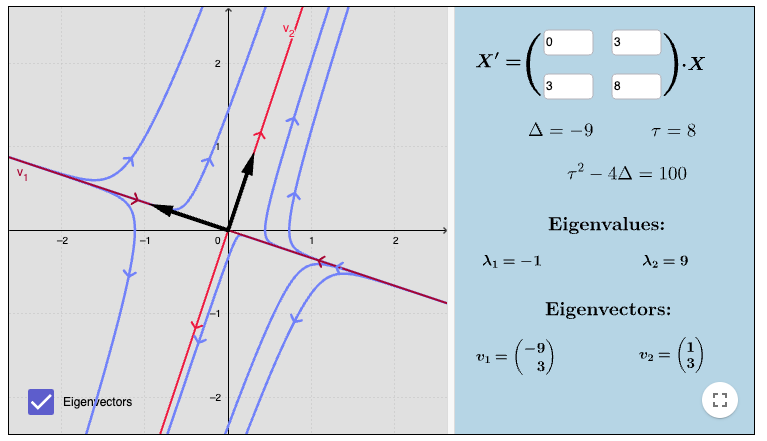
\includegraphics[width=5in]{Images/ImgPhasePlane0338.png}
    %     \end{center}         
    } 
    \else 
        \begin{center}
        \begin{tikzpicture}[scale=0.85]
        \draw[very thick, ->] (-3, 0) -- (3.25, 0);
        \draw[very thick, ->] (0, -3) -- (0, 3.25);
        \end{tikzpicture}
        \end{center}    
        \vspace{2cm}
    \fi        
\end{parts}